\documentclass[12pt]{extarticle}
\usepackage{kotex}
\usepackage{fullpage}
\usepackage{setspace}
\usepackage{amsmath}
\usepackage{amsfonts}
\usepackage{hyperref}
\usepackage{mathtools,amssymb}
\usepackage{listings}

\title{\textbf{COSE215-Assignment-Report---November 11}  \\ COSE215: Theory of Computation}

\author{\textbf{Geonho Park} \\ Department of Computer Science and Engineering, Korea University}

\hypersetup{
    colorlinks=true,
    linkcolor=blue,
    filecolor=magenta,      
    urlcolor=cyan,
}

\begin{document}
	\maketitle
    
	\section{Explanation of my code}
		\lstinputlisting[language=Octave, firstline=1, lastline=40, basicstyle=\fontsize{9pt}{4pt}\selectfont, numbers=left]{code/prob1.py}
        
		Explanation for code 1:\newline
		
		line 12에서 패턴을 입력하기 위해 input 1의 전화 번호 예시를 하나 찾아보니 +82-10-8999-9007의 꼴로 나옴을 확인했습니다. 그리하여 line12 와 같이 설정하였습니다. 자세한 설명을 하자면
		실제로 r은 raw string 으로 \texttt{\textbackslash} 을 인식시키기 위한 수단으로 입력하였습니다. 이를 이용한다면 \texttt{\textbackslash} 을 인식시키기 위하여 \texttt{\textbackslash}\texttt{\textbackslash} 을 쓰지 않아도 됩니다.
		또한 +를 인식시키기 위하여 \texttt{\textbackslash}+ 를 사용하였으며 \texttt{\textbackslash}d\{4\} 를 이용하여 4자리 숫자를 찾도록 하였습니다. 그리하여 이 과정을 통해서 얻은 matches 는 전화번호의 두 부분 즉,  앞 네 자리와 뒤 네자리 숫자가 튜플의 형태로 저장되게 됩니다.\newline

		line 17을 보면 match는 튜플로 저장되어 있으므로 각각을 얻기 위해 front, back = match의 코드를 작성하였습니다.\newline

		line 19, 20를 보면 각 front와 back은 string 타입이지만 각 자리수의 합을 구해야 하는 상황입니다. 
		그리하여 for문으로 문자열의 원소를 돌아 그 원소를 digit 이라고 하였을때 digit은 문자열이므로 int로 타입캐스팅을 하여 이를 모두 더하는 방식을 채택하였습니다.\newline

		line 22, 23에서 문제의 조건을 보았을 때 front sum 이 back sum 보다 커야 한다고 하였으니 이와 반대로 back sum이 front sum 이상일 때 continue 하도록 하여 조건을 지켰습니다.\newline

		line 25, 26, 27, 29를 보면 last를 뒤의 4자리의 제일 끝 수를 담아두는 string을 받는 용도로 임시로 선언하여 for문을 이용해 받는 과정을 통해 last값을 각 상황에서 얻을 수 있습니다. \newline
        
		얻은 last를 띄어쓰기가 없는 모드의 print를 이용하면 전체 문자열을 다 저장하고 print를 할 필요 없이 자동으로 하나씩 출력하게 되어 답이 나오게 됩니다. \newline

		\lstinputlisting[language=Octave, firstline=1, lastline=40, basicstyle=\fontsize{9pt}{4pt}\selectfont, numbers=left]{code/prob2.py}

		Explanation for code 2:\newline
		
		line 12를 보았을때 위와 r에 대한 설명은 같으므로 생략한다고 쳤을 때  앞 부분은 A부터 Z까지의 문자중 하나를 의미합니다. 즉, 대문자 알파벳을 찾으라고 하는 것과 동일합니다. + 은 1개이상의 연속으로 나오는 형태를 찾으라는 뜻으로 배운 +의 의미와 동일합니다. \texttt{\textbackslash}d의 경우에도 그냥 숫자를 의미하여 뒤에 +를 붙여 하나 이상 나오는 패턴을 감지하라고 하는 것과 동일힙니다.  즉, 전체 패턴은 하나 이상의 대문자 알파벳 뒤에 하나 이상의 숫자가 오는 형식의 문자열을 찾으라는 것과 동일합니다.\newline

		line 15, 16을 보았을 때 추출한 단어들의 첫글자를 모으기 위해 0번째 match 요소를 위에서 소개한 print 방법을 이용하여 모아서 출력하였습니다.\newline

	\section{problem solving process}
    
	1번의 문제의 경우 section 1에서 소개한 것과 같이 조건에 맞춰서 실행을 시킨다면 결과 창에 7050552 가 뜨고 이는 zip 압축 파일을 여는 과정에서 비밀번호로 입력했을 때 답이 맞음을 확인했습니다. \newline

	2번의 경우 동일하게 실행을 시켰을 때 결과 창에 \newline
	
	IXQQBUHJXODUHASUHVVLRQ \newline
	
	가 뜸을 알 수 있었습니다. 안내 사진에 있는 내용처럼 말이 되지 않은 문장이 나오게 되어 추가적인 공정을 해야 됨을 알 수 있습니다. \newline

	실제로 Hint에 The Roman general Caesar created a cipher to comunicate with his allies 라고 되어 쓰여 있으므로 이는 카이사르 암호화가 되어 있었음을 유추할 수 있었습니다.\newline

	그럼 IXQQBUHJXODUHASUHVVLRQ 를 복호화 하여 값을 얻어내야 하는데 카이사르 복호화를 해주는 사이트가 있었습니다. \newline

	goto website \href{https://jo-gunhee.github.io/website1/dcode/dcodewebsite.html}{Link}\newline

	이 사이트에 실제로 가서 저 문장을 입력해본다면 \newline

	%\begin{figure}[h]
    %    \centering
    %     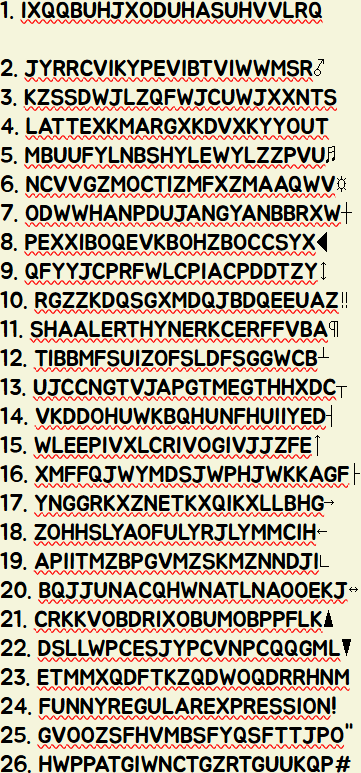
\includegraphics[width=0.4\textwidth]{image/web.png}
    % \end{figure}

	FUNNYREGULAREXPRESSION\newline

    이 나옴을 확인해볼 수 있습니다. 실제로 !가 같이 떠서 나오긴 하지만 원문보다 글자수가 하나 넘어서는 것을 보니 오류로 생각하였습니다. \newline
	
	
	\section{results}

	1번 답은 7050552, 2번 답은 FUNNYREGULAREXPRESSION 이 떴음을 확인하였습니다 \newline

	이 과정을 통해 re module 에 대한 더 심층적인 이해가 가능하게 되었습니다. 

\end{document}